\section{Esamų sistemų pertvarkymas}
Apibrėžus šablonus paketų skirstymui galima pradėti vertinti jų įtaką sistemai, juos pritaikant esamoms sistemoms.
Šio skyriaus tikslas - pasirinkti ir išnagrinėti kelias sistemas pasitelkus paketų kokybės matus bei bendrą sistemos struktūros analizę,
taip identifikuojant programiniam kodui būdingas problemas, rastas problemas išspręsti pritaikant aprašytus šablonus.
Atlikus pertvarkymus sistemose, dar kartą paskaičiuoti paketų kokybės matus,
taip gaunant įrodymus, ar gauti šablonai yra efektyvūs ir iš tiesų sprendžia
jiems priskirtas problemas.


\subsection{Sistemų pasirinkimas}
Sistemų pertvarkymui pasirinktos atviro kodo sistemos, kurių kodas yra viešai prieinamas \textit{github} platformoje.
Pasirinktos sistemos yra vidutinio dydžio, todėl nėra labai sudėtinga jas suprasti ir pertvarkyti, bet taip pat jos nėra
tokios paprastos, kad neturėtų sistemos dizaino problemų.
Pasirinktos sistemos yra skirtingo tipo projektai, taip užtikrinant didesnę problemų ivairovę ir objektyvesnius įvertinimus.
Per visą pasirinktų sistemų imtį yra sutinkamos visos aprašytos problemos, taip įvertinant visus aprašytus šablonus.

\subsection{\textit{crawler4j} sistema}
\textbf{crawler4j\footnote{\url{https://github.com/yasserg/crawler4j}}} yra atvirojo kodo
žiniatinklio tikrinimo \angl{crawling} programa parašyta \textit{Java} programavimo kalba, leidžianti
efektyviai tikrinti žiniatinklį naudojant daugiagijį angl{multithreaded} metodą.
Tai taikomosios programinės įrangos tipas, skirtas vartotojams.

Prieš visus pakeitimus \textit{crawler4j} sistemos paketų struktūra atrodo taip:
\begin{figure}[H]
    \centering
    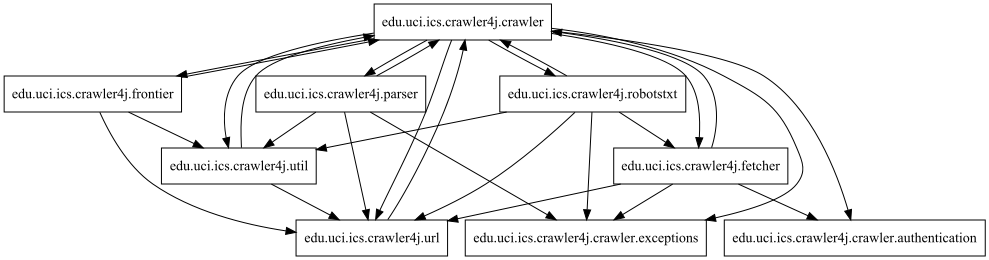
\includegraphics[scale=0.5]{img/crawler_packages_orig}
    \caption{\textit{crawler4j} sistemos struktūra}
    \label{img:crawler_packages_orig}
\end{figure}

Atlikus sistemos kokybės matų analizę galima pamatyti sistemai būdingas problemas:
\begin{center}
    \begin{tabular}{|c|c|c|c|c|c|c|c|}
        \hline
        Paketo vardas & \textit{N} & \textit{A} & \textit{E} & \textit{S} & \textit{A} & \textit{D} & \textit{C} \\ [0.5ex]
        \hline\hline
        edu.uci.ics.crawler4j.crawler.authentication & 4 & 2 & 0 & 0.0 & 0.25 & 0.75 & 0\\
        \hline
        edu.uci.ics.crawler4j.url & 4 & 6 & 1 & 0.143 & 0.0 & 0.857 & 1 \\
        \hline
        edu.uci.ics.crawler4j.crawler.exceptions & 3 & 4 & 0 & 0.0 & 0.0 & 1.0 & 0\\
        \hline
        edu.uci.ics.crawler4j.crawler & 5 & 6 & 8 & 0.571 & 0.2 & 0.229 & 5 \\
        \hline
        edu.uci.ics.crawler4j.robotstxt & 6 & 1 & 5 & 0.833 & 0.0 & 0.167 & 1 \\
        \hline
        edu.uci.ics.crawler4j.frontier & 6 & 1 & 3 & 0.75 & 0.0 & 0.25 & 1 \\
        \hline
        edu.uci.ics.crawler4j.fetcher & 6 & 2 & 4 & 0.667 & 0.0 & 0.333 & 1 \\
        \hline
        edu.uci.ics.crawler4j.util & 3 & 4 & 2 & 0.333 & 0.0 & 0.667 & 0 \\
        \hline
        edu.uci.ics.crawler4j.parser & 12 & 1 & 4 & 0.8 & 0.167 & 0.033 & 1 \\
        \hline
    \end{tabular}
    \begin{tabular}{|c|c|c|c|c|c|c|}
        \hline
        $\bar{N}$ & $\bar{Af}$ & $\bar{Ef}$ & $\bar{S}$ & $\bar{A}$ & $\bar{D}$ & $\Sigma C$  \\ [0.5ex]
        \hline\hline
        5 & 3 & 3 & 0.455 & 0.069 & 0.476 & 5\\
        \hline
    \end{tabular}
\end{center}
Iš bendros sistemos analizės bei matų lentelės rezultatų matomos kelios sistemos problemos -
\begin{itemize}
    \item \textbf{Problema numeris 1} - atlikus bendrą sistemos kodo analizę matoma,
    kad sistemos paketuose yra daug sąsajų su skirtingais jų įgyvendinimais, todėl yra sunku
    rasti visus specifinės sąsajos įgyvendinimus, esama paketų struktūra tam nepadeda
    \item \textbf{Problema numeris 2} - paketo \textit{edu.uci.ics.crawler4j.parser} viduje yra 12 klasių, todėl sunku suprasti už kokius funkcionalumus jis atsakingas
    ir kada jį reikėtų nagrinėti bei keisti.
    \item \textbf{Problema numeris 3} - Sistema turi daug ciklinių prilausomynbių, kur du arba daugiau paketų priklauso vienas nuo kito.
    Tai aiškiai matosi sistemos paketų diagramoje\ref{img:crawler_packages_orig}, ciklinėse priklausomybėse išviso dalyvauja 10 paketų ir kartu jie sudaro 5 ciklinių priklausomybių sekas,
    kurios turėtų būti pašalintos.
\end{itemize}

Sistemos paketas \textit{edu.uci.ics.crawler4j.parse}, turi sąsają \textit{ParseData} bei 4 skirtingųs jos įgyvendinimus - \textit{CssParseData, TextParseData, HtmlParseData, BinaryParseData},
šios klasės pakete dalinasi vieta dar su 9 klasėmis, todėl yra gan nepatogu rasti ieškomą įgyvendinimą.
\begin{figure}[H]
    \snugshade
    \dirtree{%
        .1 {/parser} .
        .2 {AllTagMapper}.
        .2 {ParseData}.
        .3 {TextParseData}.
        .3 {HtmlParseData}.
        .2 {CssParseData}.
        .2 {BinaryParseData}.
        .2 {ExtractedUrlAnchorPair}.
        .2 {HtmlParser}.
        .2 {HtmlContentHandler}.
        .2 {TikaHtmlParser}.
        .2 {Parser}.
    }
    \endsnugshade
    \caption{\textit{parser} paketo struktūra}
\end{figure}
Šiam paketui sutvarkyti taikomas \textit{Sąsajų atskyrimo} šablonas - sąsaja iškeliama į atskirą paketą \textit{parse}, jos įgyvendinimai perkliami į minėto
paketo subpaketus.
Šie pertvarkymai pakeičia \textit{parser} paketo struktūrą:
\begin{figure}[H]
    \snugshade
    \dirtree{%
        .1 {/parser} .
        .2 {parse}.
        .3 {ParseData // Sąsaja}.
        .3 {text}.
        .4 {TextParseData // Pirmas sąsajos įgyvendinimas}.
        .3 {html }.
        .4 {HtmlParseData // Antras sąsajos įgyvendinimas}.
        .3 {css }.
        .4 {CssParseData // Trečias sąsajos įgyvendinimas}.
        .3 {binary}.
        .4 {BinaryParseData // Ketvirtas sąsajos įgyvendinimas}.
        .2 {AllTagMapper}.
        .2 {ExtractedUrlAnchorPair}.
        .2 {HtmlParser}.
        .2 {HtmlContentHandler}.
        .2 {NotAllowedContentException}.
        .2 {TikaHtmlParser}.
        .2 {Parser}.
    }
    \endsnugshade
    \caption{\textit{parser} paketo struktūra po pirmojo pertvarkymo}
\end{figure}
Dėl atskirtos sąsajos ir jos įgyvendinimų tampa daug paprasčiau ją rasti bei suprasti sistemoje egzistuojančius jos įgyvendinimus.
Tokia struktūra išsprendžia sistemos \textbf{problemą numeris 1}.
Šis pertvarkymas taip dalinai sumažino \textbf{problemą numeris 2}, sumažinant klasių skaičių pakete į 7.
Palyginus pertvarkytos ir buvusios sitemos matus matome, kad sistema tapo aiškesnė, sumažėjo vidutinis klasių skaičius paketuose, tačiau neženkliai nukrito
vidutinis stabilumas ir abstrakcijos lygis, todėl atstumas nuo pagrindinės sekos nežymiai padidėjo.
\begin{center}
    \begin{tabular}{|c|c|c|c|c|c|c|c|}
        \hline
        \textit{crawler4j.parser} & \textit{N} & \textit{A} & \textit{E} & \textit{S} & \textit{A} & \textit{D} & \textit{C} \\ [0.5ex]
        \hline\hline
        Prieš & 12 & 1 & 4 & 0.8 & 0.167 & 0.033 & 1 \\
        \hline
        Po & \cellcolor{green!25} 7 (-5) & 1 & 9 & \cellcolor{red!25} 0.9 + (0.1) & \cellcolor{red!25} 0.143 (-0.024) & \cellcolor{red!25} 0.043 (+0.01) & 1 \\
        \hline
    \end{tabular}
    \begin{tabular}{|c|c|c|c|c|c|c|c|}
        \hline
        Vidurkiai & $\bar{N}$ & $\bar{Af}$ & $\bar{Ef}$ & $\bar{S}$ & $\bar{A}$ & $\bar{D}$ & $\Sigma C$ \\ [0.5ex]
        \hline\hline
        Prieš & 5 & 3 & 3 & 0.455 & 0.069 & 0.476 & 5\\
        \hline
        Po & \cellcolor{green!25}  4 (-1) & 3 & 3 & \cellcolor{red!25} 0.488 (+0.033) & \cellcolor{green!25} 0.114 (+0.045) & \cellcolor{green!25} 0.425 (-0.051) & 5 \\
        \hline
    \end{tabular}
\end{center}
Norint išspręsti \textbf{problemą numeris 3} - ciklines priklausomybes, reikia identifikuoti klases, kurių priklausomybės
sudaro ciklus ir iškelti jas į atskirus paketus.
todo: pridėti citavimą iš straipsnio apie ciklinių priklausomybių eliminavimą

Kuriant naujus paketus vadovaujamasi \textit{skirstymo pagal teikiamą funkcionalumą} šablonu, užtikrinant, kad kiekvienas
paketas teikia vieną, aiškiai apibrėžtą funkciją, kuri yra pasiekiama per pakete aprašytą sąsają.
Paketo vidus yra paslėptas su \textit{Java} kalbos pasiekiamumo modifikatoriais - konkrečių klasių negalima inicializuoti už paketo ribų,
nes jų konstruktoriai privatūs.
Sąsajos įgyvendinimas gaunamas \textit{static factory} pagalba.
todo: aprašyti, kas tai yra

\begin{figure}[H]
    \begin{lstlisting}[language=Python]
public interface HtmlParser {

    HtmlParseData parse(ParsedPage page, String contextURL) throws ParseException;

    // Grąžinamas sąsajos įgyvendinimas
    static HtmlParser newHtmlParser(CrawlConfig config, TLDList tldList) throws InstantiationException, IllegalAccessException  {
        return new TikaHtmlParser(config, tldList);
    }
}

// Sąsajos įgyvendinimas. Nėra viešas, pasiekiamas tik paketo viduje,
// nes klasė ir konstruktorius nenaudoja public raktažodžių
class TikaHtmlParser implements HtmlParser {
   ...
    TikaHtmlParser(CrawlConfig config, TLDList tldList) throws InstantiationException, IllegalAccessException {
     ...
    }
    \end{lstlisting}
    \caption{\textit{skirstymo pagal teikiamą funkcionalumą} šablono sąsaja}
\end{figure}
Peržiūrėjus paketus su ciklinėmis priklausomybės, iš jų buvo išskirti šie nauji funkcionalumai, kuriems
buvo sukurti atskiri paketai:
\begin{itemize}
    \item Iš \textit{parser} paketo iškeltas funkcionalumas \textit{html} turiniui apdoroti, patalpintas į \textit{parser/html} paketą.
    Po šio pertvarkymo \textit{parser} paketas pasidaro pakankamai mažas ir turi vieną funkcionalumą - priimti puslapį ir deleguoti jį apdorojimui kitai klasei pagal puslapio tipą.
    \item Iš \textit{robotstxt} paketo funkcionalumas patikrinti ar sistema autorizuota apdoroti pasirinktą puslapį iškeltas į \textit{robotstxt/permissions} paketą.
    \item Iš \textit{crawler}, bei \textit{parser} paketų funkcionalumas programiškai aprašantis internetinio puslapio elementus iškeltas į \textit{web} paketą.
    \item Iš \textit{crawler} paketo funkcionalumas nustatyti įrankio konfigūraciją iškeltas į \textit{config} paketą.
    \item Iš \textit{url} paketo funkcionalumas gauti internetinių domenų pavadinimus iškeltas į \textit{tld} paketą.
\end{itemize}

\begin{figure}[H]
    \snugshade
    \dirtree{%
        .1 {/} .
        .2 {crawler4j}.
        .3 {crawler}.
        .4 {authentication}.
        .4 {exceptions}.
        .3 {fetcher}.
        .3 {frontier}.
        .3 {parser}.
        .4 {parse}.
        .5 {binary}.
        .5 {css}.
        .5 {factory}.
        .5 {html}.
        .5 {text}.
        .3 {robotstxt}.
        .3 {url}.
        .3 {util}.
    }
    \endsnugshade
    \caption{\textit{crawler4j} paketų medis prieš iškeliant minėtus funkcionalumus}
\end{figure}

\begin{figure}[H]
    \snugshade
    \dirtree{%
        .1 {/} .
        .2 {crawler4j}.
        .3 {config}.
        .3 {crawler}.
        .4 {authentication}.
        .3 {fetcher}.
        .3 {frontier}.
        .3 {parser}.
        .4 {html}.
        .4 {parse}.
        .5 {binary}.
        .5 {css}.
        .5 {html}.
        .5 {text}.
        .3 {robotstxt}.
        .4 {permissions}.
        .3 {tld}.
        .3 {util}.
        .3 {web}.
    }
    \endsnugshade
    \caption{\textit{crawler4j} paketų medis iškėlus minėtus funkcionalumus}
\end{figure}

Atlikus šiuos funkcionalumų suskaidymus į atskirus paketus buvo panaikintos žiedinės priklausomybės.
Naujoje paketų diagramoje galime matyti, jog dabar sistema turi daug daugiau paketų, tačiau jų priklausomybių kryptys daug aiškesnės:
\subsection{\textit{Crawler} sistema}
\begin{figure}[H]
    \centering
    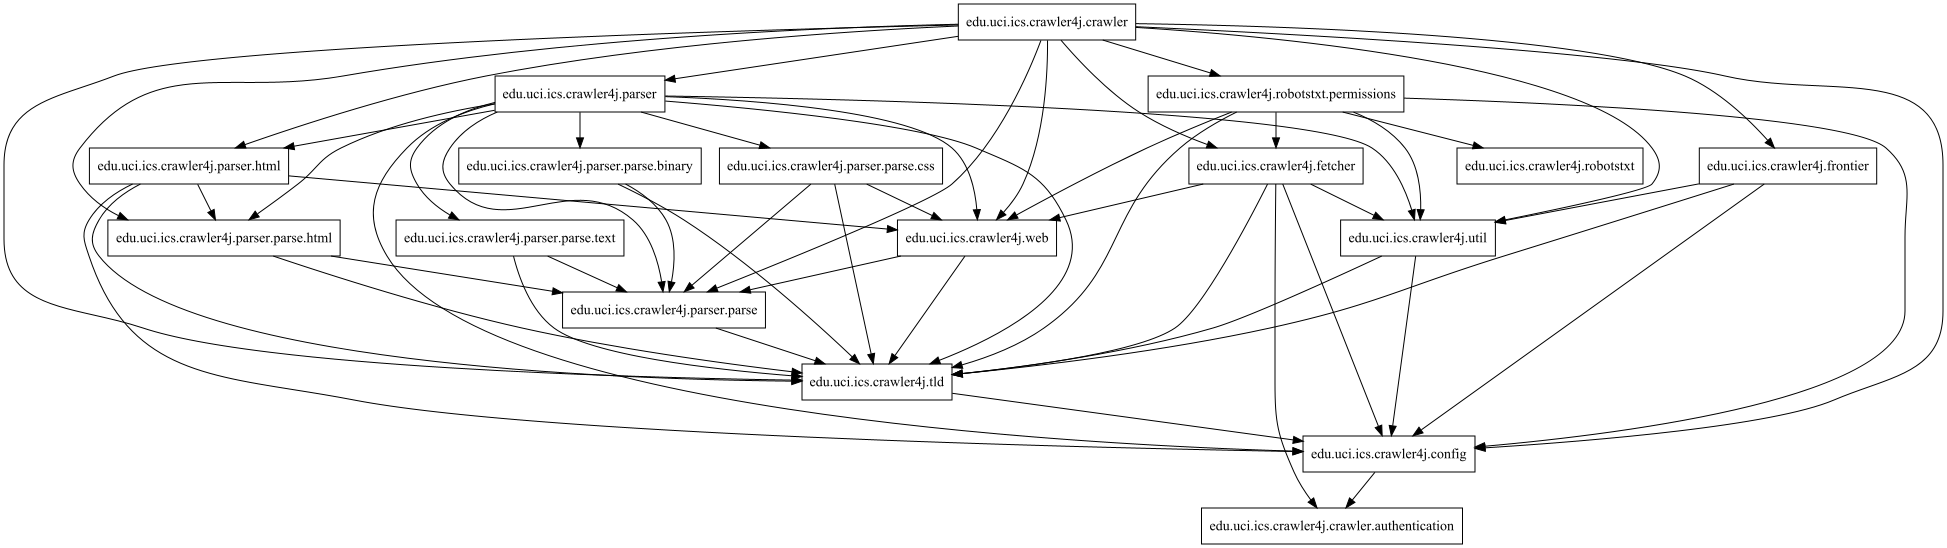
\includegraphics[scale=0.2]{img/crawler_packages_v2}
    \caption{\textit{crawler4j} sistemos struktūra po antro pertvarkymo}
    \label{img:crawler_packages_v2}
\end{figure}
todo: ranka perpiešti sugeneruotus paveikslėlius, kad jie geriau tilptų į puslapį

Atlikus matų analizę pertvarkytai sistemai yra matoma, kad sistemos kokybė pagerėjo,
sumažėjo vidutinis klasių skaičius pakete, ciklinių priklausomybių rodiklis tapo lygus nuliui,
padidėjo vidutinis abstrakcijos lygis:
\begin{center}
    \begin{tabular}{|c|c|c|c|c|c|c|c|}
        \hline
        Paketo vardas & \textit{N} & \textit{Af} & \textit{Ef} & \textit{S} & \textit{A} & \textit{D} & \textit{C} \\ [0.5ex]
        \hline\hline
        edu.uci.ics.crawler4j.parser.parse.binary & 1 & 1 & 2 & 0.667 & 0.0 & 0.333 & 0 \\
        \hline
        edu.uci.ics.crawler4j.crawler & 4 & 0 & 11 & 1.0 & 0.25 & 0.25 & 0 \\
        \hline
        edu.uci.ics.crawler4j.tld & 3 & 13 & 1 & 0.071 & 0.333 & 0.596 & 0 \\
        \hline
        edu.uci.ics.crawler4j.parser.html & 6 & 2 & 4 & 0.667 & 0.167 & 0.166 & 0 \\
        \hline
        edu.uci.ics.crawler4j.robotstxt.permissions & 2 & 1 & 6 & 0.857 & 0.5 & 0.357 & 0 \\
        \hline
        edu.uci.ics.crawler4j.config & 1 & 8 & 1 & 0.111 & 0.0 & 0.889 & 0 \\
        \hline
        edu.uci.ics.crawler4j.frontier & 6 & 1 & 3 & 0.75 & 0.0 & 0.25 & 0 \\
        \hline
        edu.uci.ics.crawler4j.parser & 2 & 1 & 10 & 0.909 & 0.0 & 0.091 & 0\\
        \hline
        edu.uci.ics.crawler4j.crawler.authentication & 4 & 2 & 0 & 0.0 & 0.25 & 0.75 & 0 \\
        \hline
        edu.uci.ics.crawler4j.parser.parse.css & 1 & 1 & 3 & 0.75 & 0.0 & 0.25 & 0 \\
        \hline
        edu.uci.ics.crawler4j.robotstxt & 5 & 1 & 0 & 0.0 & 0.0 & 1.0 & 0 \\
        \hline
        edu.uci.ics.crawler4j.parser.parse.html & 1 & 3 & 2 & 0.4 & 0.0 & 0.6 & 0 \\
        \hline
        edu.uci.ics.crawler4j.parser.parse & 1 & 7 & 1 & 0.125 & 1.0 & 0.125 & 0\\
        \hline
        edu.uci.ics.crawler4j.fetcher & 6 & 2 & 5 & 0.714 & 0.0 & 0.286 & 0 \\
        \hline
        edu.uci.ics.crawler4j.util & 4 & 5 & 2 & 0.286 & 0.0 & 0.714 & 0 \\
        \hline
        edu.uci.ics.crawler4j.web & 5 & 6 & 2 & 0.25 & 0.4 & 0.35 & 0 \\
        \hline
        edu.uci.ics.crawler4j.parser.parse.text & 1 & 1 & 2 & 0.667 & 0.0 & 0.333 & 0 \\
        \hline
    \end{tabular}
    \begin{tabular}{|c|c|c|c|c|c|c|c|}
        \hline
        Vidurkiai & $\bar{N}$ & $\bar{Af}$ & $\bar{Ef}$ & $\bar{S}$ & $\bar{A}$ & $\bar{D}$ & $\Sigma C$ \\ [0.5ex]
        \hline\hline
        Prieš & 5 & 3 & 3 & 0.455 & 0.069 & 0.476 & 5\\
        \hline
        Po  & \cellcolor{green!25} 3 (-2) & 3 & 3 & \cellcolor{green!24} 0.452 (-0.03) & \cellcolor{green!25} 0.183 (+0.114) & \cellcolor{green!25} 0.471 (-0.005) & \cellcolor{green!25} 0 (-5)\\
        \hline
    \end{tabular}
\end{center}
Iš gautų rezultatų galime teigti jog po pertvarkymo galima teigti, kad šablonai \textit{skirstymas pagal teikiamą funkcionalumą} ir \textit{sąsajų atskyrimas}, išsprendė visas 3 sistemoje matytas problemas,
padarė sistemą lengviau suprantamą žmogui, panaikino ciklines priklausomybes, ir turėjo teigiama įtaka matams, nurodantiems
sistemos įgyvendinimo kokybę.


\subsection{\textit{azure-sdk-for-java} sistema}
\textbf{azure-sdk-for-java\footnote{\url{https://github.com/Azure/azure-sdk-for-java/tree/main/sdk/storage/azure-storage-blob-cryptography}}} yra atvirojo kodo
biblioteka, parašyta \textit{Java} programavimo kalba, leidžianti programiškai bendrauti su \textit{Microsoft Azure} debesų kompiuterijos platforma.
Tai programinės įrangos įrankis, skirtas naudoti kitose sistemose supaprastinant programinį kodą.
Ši biblioteka yra labai didelė ir šio pertvarkymo metu yra dirbama tik su posistemė \textit{azure-storage-blob-cryptograph}, kuri atsakingą už duomenų kriptografiją,
komunikacijos su \textit{Azure Blog} nestruktūrizuota failų saugykla metu

Prieš visus pakeitimus \textit{azure-storage-blob-cryptograph} sistema turi vieną paketą \textit{com.azure.storage.blob.specialized.cryptography}, kuriame guli visos jos klasės.

Sistemos kokybės matai nėra naudingi dirbant su vienų paketų, nes trūksta konteksto suprasti kaip paketas yra naudojamas.
Tačiau iš bendrines sistemos analizės galima pamatyti pagrindines sistemos problemas - viename pakete yra 21 skirtinga klasė, tiek sąsajos, tiek konrkečios klasės.
Taip sistemoje yra kelios skirtingos tos pačios esybės versijos - \textit{DecryptorV1} ir \textit{DecryptorV2}, \textit{EncryptorV1} ir \textit{EncryptorV2}, dėl ko yra sunku
suprasti kokios klasės su kokią esybės versija yra susijusios, bei yra papildomo kodo pasikartojimo.
Ši sistema būtų aiškesnę ir greičiau perprantama jei būtų išskirti mažesni funcionalumai ir pagal juos kodas išskaidytas į smulkesnius paketus, taip pat atskyriant juos
pagal esybių versijas.
Kad atlikti teisingą esybių versijavima naudojamas \textit{atskirų versijų skirstymo} šablonas, pagal jį kiekvienai esybės versijai sukuriamas po atskiras paketas,
taip pat bendras, pasikartojantis kodas iškeliamas į abstrakčia klasę, kuri yra padėta pakete, vienu lygiu auksčiau nei versijų paketai:
\begin{figure}[H]
    \snugshade
        \dirtree{%
            .1 {/cryptography} .
            .2 {decryptor} .
            .3 {Decryptor  // Abstrakti klasė su bendru esybės kodu} .
            .3 {v1} .
            .4 {DecryptorV1 // Pirma esybės versija} .
            .3 {v2} .
            .4 {DecryptorV2 // Antra esybės versija} .
            .2 {encryptor} .
            .3 {Encryptor  // Abstrakti klasė su bendrų esybės kodu} .
            .3 {agent // Papildomas su esybę susijes kodas, naudojamas abieju esybių} .
            .3 {v1} .
            .4 {EncryptorV1 // Pirma esybės versija} .
            .3 {v2} .
            .4 {EncryptorV2 // Antra esybės versija} .
        }
    \endsnugshade
    \caption{\textit{azure-storage-blob-cryptograph} paketų medis su paketais, dedikuotais esybių versijų valdymui}
\end{figure}
Šis pakeitimas, pagal \textit{atskirų versijų skirstymo} šabloną, atskyria esybes versijas ir pristato kelis paketus apibrėžiančius aiškesnius funkcionalumus,
kadangi atsirado daugiau paketų bei saveiką tarp jų galima paskaičiuoti paketų kokybės matus:
\begin{center}
    \begin{tabular}{|c|c|c|c|c|c|c|c|}
        \hline
        Paketo vardas & \textit{N} & \textit{Af} & \textit{Ef} & \textit{S} & \textit{A} & \textit{D} & \textit{C} \\ [0.5ex]
        \hline\hline
        specialized.cryptography & 13 & 7 & 5 & 0.417 & 0.0 & 0.583 & 5 \\
        \hline
        specialized.cryptography.encryptor.v2 & 1 & 1 & 3 & 0.75 & 0.0 & 0.25 & 0 \\
        \hline
        specialized.cryptography.encryptor.v1 & 1 & 0 & 3 & 1.0 & 0.0 & 0.0 & 1 \\
        \hline
        specialized.cryptography.encryptor & 1 & 4 & 2 & 0.333 & 1.0 & 0.333 & 2 \\
        \hline
        specialized.cryptography.decryptor.v2 & 1 & 1 & 2 & 0.667 & 0.0 & 0.333 & 1 \\
        \hline
        specialized.cryptography.decryptor.v1 & 1 & 1 & 2 & 0.667 & 0.0 & 0.333 & 1\\
        \hline
        specialized.cryptography.encryptor.agent & 2 & 3 & 2 & 0.4 & 0.0 & 0.6 & 1\\
        \hline
        specialized.cryptography.decryptor & 2 & 3 & 1 & 0.25 & 0.5 & 0.25 & 1 \\
        \hline
    \end{tabular}
    \begin{tabular}{|c|c|c|c|c|c|c|}
        \hline
        $\bar{N}$ & $\bar{Ag}$ & $\bar{Eg}$ & $\bar{S}$ & $\bar{A}$ & $\bar{D}$ & $\Sigma C$ \\ [0.5ex]
        \hline\hline
        3 & 3 & 3 & 0.561 & 0.188 & \cellcolor{green!25} 0.335 & \cellcolor{red!25} 6 \\
        \hline
    \end{tabular}
\end{center}
Apskaičiuoti matai rodo nedidelį nuokrypį nuo pagrindinės sekos, todėl galima teigti kad sistemos abstraktumas bei stabilumas
yra subalansuoti, tačiau šiš skirstymas turėjo ir neigiamu padaryniu - sukelė 5 cilines priklausomybes.
Šiais ciklines priklausomybes galima aiškiai matyti sistemos paketų diagramoje:
\begin{figure}[H]
    \centering
    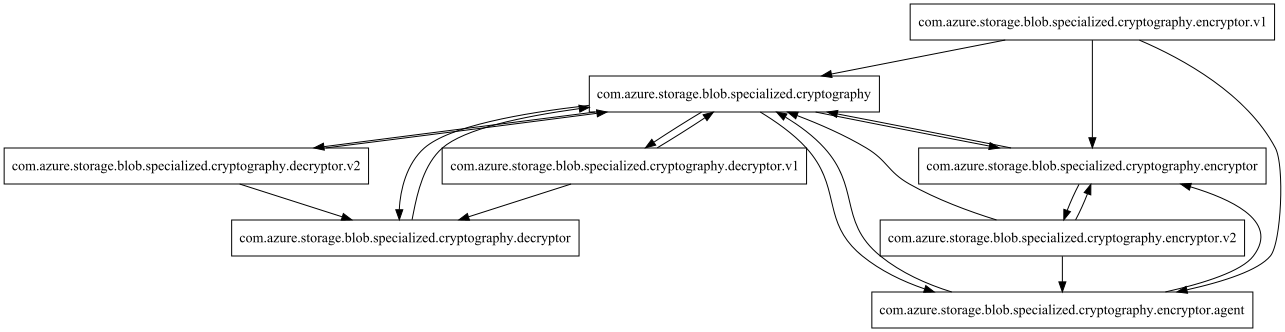
\includegraphics[scale=0.3]{img/azure_packages_v1}
    \caption{\textit{azure-storage-blob-cryptograph} sistemos struktūra po pirminio pertvarkymo}
    \label{img:azure_packages_v1}
\end{figure}
Tam, kad panaikinti ciklines priklausomybes reikia panaudoti šablona \textit{skirstymas pagal teikiamą funkcionalumą} ir išskaidant pagrindinį paketą,
dar į smulkesnius vienetus - yra sukuriamas paketas \textit{encription.data} paketas, atsakingas programiškai atvaizduoti užkoduotus duomenis, taip pat
aprašomas paketas \textit{blob} skirtas \textit{blob} esybes, reprezentuojančios saugyklos duomenų formatą, kriptografijai.
Taip pat vadovaujantys \textit{pagalbinių klasių priskyrimas dalykinės srities paketui} šablonu, visos pagalbinės klasės, neturinčios priklausomybių į kitus paketus ir
padedančios vykdyti kertinius funcionalumus yra iškeliamos į \textit{util} paketą.
Minėtame pakete atsiranda tokios klasės:
\begin{itemize}
    \item \textit{CryptographyConstants} - klasė saugojanti bendras su kriptografija susijusias konstantas, kurios naudojamos skirtingose vietose sistemoje.
    \item \textit{EncryptionVersion} - Aprašo kriptografijos versijas ir jų naudojamus protokolos
    \item \textit{WrappedKeyJson} - palengvina darbą su serializuojant ir deserializuojant kriptografijos raktus į \textit{json} formatą.
\end{itemize}

Pritaikius visus šiuos šablonus, gaunama sistemos struktūra su nedideliais, aiškesniais funkcionalumais apibrėžtais paketais, taip pat yra pašalinamos ciklinės priklausomybės:
\begin{figure}[H]
    \centering
    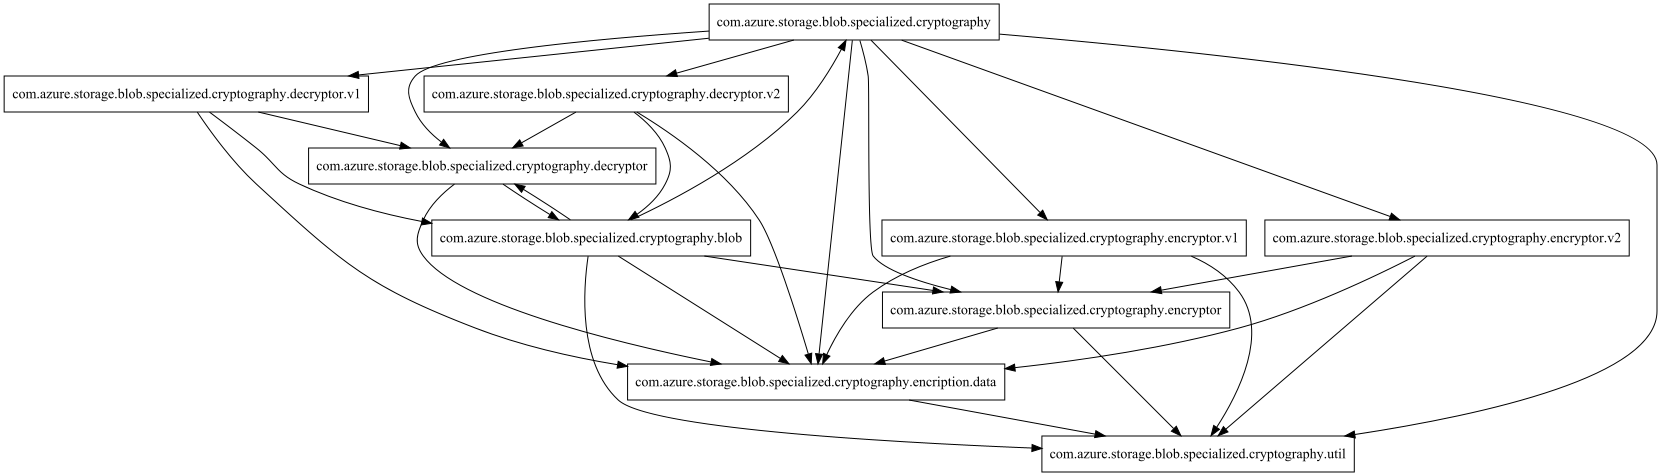
\includegraphics[scale=0.35]{img/azure_packages_v2}
    \caption{Galutinė \textit{azure-storage-blob-cryptograph} sistemos struktūra}
    \label{img:azure_packages_v2}
\end{figure}

Išnaujo įvertinus matus, matoma, kad nuokrypis pagrindinės sekos šiek tiek padidėjo, tačiau
vistiek yra gan mažas, ciklinės priklausomybės išnyko, todėl galime teigti, kad \textit{skirstymo pagal teikiamą funkcionalumą},
\textit{pagalbinių klasių priskyrimo} ir \textit{atskirų versijų skirstymo} šablonai prisidėjo prie bendro
sistemos suprantamumo, įvedė aiškesnę jos struktūrą, išlaikant objektyviai gerus sistemos kokybės matus.
\begin{center}
    \begin{tabular}{|c|c|c|c|c|c|c|c|}
        \hline
        Paketo vardas & \textit{N} & \textit{Af} & \textit{Ef} & \textit{S} & \textit{A} & \textit{D} & \textit{C} \\ [0.5ex]
        \hline\hline
        specialized.cryptography & 3 & 1 & 8 & 0.889 & 0.0 & 0.111 & 0 \\
        \hline
        specialized.cryptography.blob & 6 & 3 & 5 & 0.625 & 0.0 & 0.375 & 0 \\
        \hline
        specialized.cryptography.encription.data & 4 & 8 & 1 & 0.111 & 0.0 & 0.889 & 0 \\
        \hline
        specialized.cryptography.encryptor.v2 & 1 & 1 & 3 & 0.75 & 0.0 & 0.25 & 0 \\
        \hline
        specialized.cryptography.encryptor.v1 & 1 & 1 & 3 & 0.75 & 0.0 & 0.25 & 0 \\
        \hline
        specialized.cryptography.encryptor & 1 & 4 & 2 & 0.333 & 1.0 & 0.333 & 0 \\
        \hline
        specialized.cryptography.decryptor.v2 & 1 & 1 & 3 & 0.75 & 0.0 & 0.25 & 0 \\
        \hline
        specialized.cryptography.decryptor.v1 & 1 & 1 & 3 & 0.75 & 0.0 & 0.25 & 0 \\
        \hline
        specialized.cryptography.decryptor & 2 & 4 & 2 & 0.333 & 0.5 & 0.167 & 0 \\
        \hline
        specialized.cryptography.util & 3 & 6 & 0 & 0.0 & 0.0 & 1.0 & 0 \\
        \hline
    \end{tabular}
    \begin{tabular}{|c|c|c|c|c|c|c|c|}
        \hline
        Vidurkiai & $\bar{N}$ & $\bar{A}$ & $\bar{E}$ & $\bar{S}$ & $\bar{A}$ & $\bar{D}$ & $\Sigma C$ \\ [0.5ex]
        \hline\hline
        Pirmas pertvarkymas & 3 & 3 & 3 & 0.561 & 0.188 & 0.335 &  6 \\
        Galutinis variantas & \cellcolor{green!25} 2 (-1) & 3 & 3 & \cellcolor{green!25} 0.529 (-0.032) & \cellcolor{red!25} 0.15 (-0.03) & \cellcolor{red!25} 0.388 (+0.053) &  \cellcolor{green!25} 0 (-5) \\
        \hline
    \end{tabular}
\end{center}

todo: parasyti bendras isvadas
todo: parašyti, pertvarkymo tikslas nėra gerinti matus, o jie yra naudojami norint įsitikinti, jog kokybė nesuprastejo. Šiuo atveju svarbiau skaitomumas, o ne kokybė paremta matais
todo: paaiškinti metricas
todo: sutvarkyti izanga